
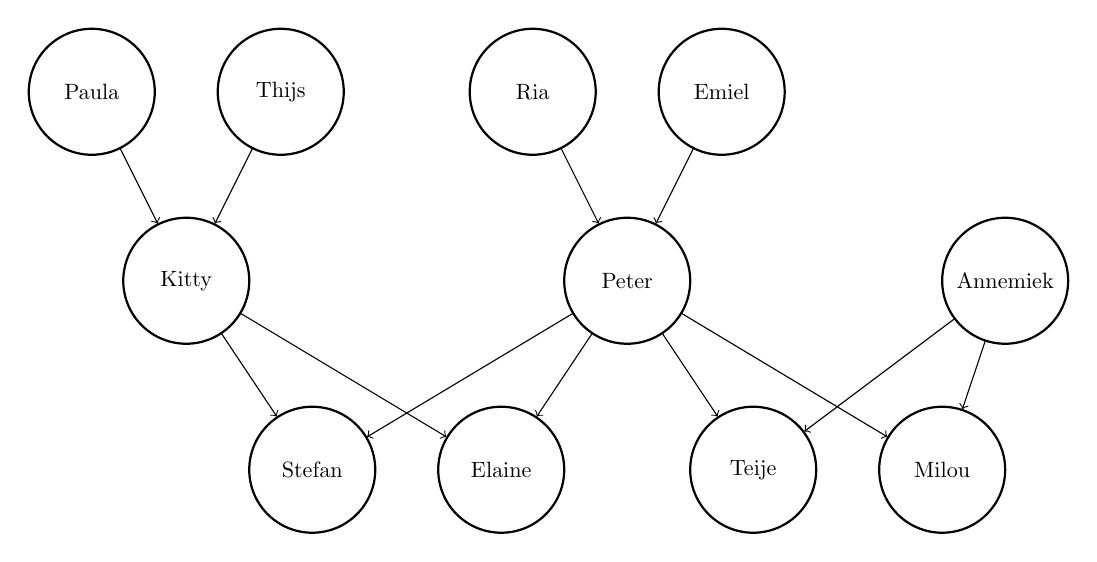
\begin{tikzpicture}[scale=0.8, transform shape]
	\begin{scope}[every node/.style={circle,thick,draw, minimum size = 2cm}]
		\node[] (Paula) at (0,0) {Paula};
    \node (Thijs) at (3,0) {Thijs};
    \node[] (Ria) at (7,0) {Ria};
		\node[] (Emiel) at (10,0) {Emiel};
		\onslide<3->{
    \node (Kitty) at (1.5,-3) {Kitty};
    \node (Peter) at (8.5,-3) {Peter};
		\onslide<4->{
    \node (Stefan) at (3.5,-6) {Stefan};
    \node (Elaine) at (6.5,-6) {Elaine};
	}
	}
		\onslide<5->{
    	\node (Annemiek) at (14.5,-3) {Annemiek};
			\node (Teije) at (10.5,-6) {Teije};
			\node (Milou) at (13.5,-6) {Milou};
		}
\end{scope}

\begin{scope}[
              every node/.style={fill=white,circle},
							every edge/.style={draw=black}]
							\onslide<3->{
							\path[->] (Paula) edge (Kitty); 
							\path[->] (Thijs) edge (Kitty); 
							\path[->] (Ria) edge (Peter); 
							\path[->] (Emiel) edge (Peter); 
						}
						\onslide<4->{
							\path[->] (Kitty) edge (Stefan); 
							\path[->] (Peter) edge (Stefan); 
							\path[->] (Kitty) edge (Elaine); 
							\path[->] (Peter) edge (Elaine); 
						}
							\onslide<5->{

							\path[->] (Annemiek) edge (Teije); 
							\path[->] (Peter) edge (Teije); 
							\path[->] (Annemiek) edge (Milou); 
							\path[->] (Peter) edge (Milou); 
							}
\end{scope}
\end{tikzpicture}
